\section{Mô phỏng thiết kế}

\subsection{Môi trường mô phỏng}
Testbench Verilog có sẵn trong RD1139: gồm model bus, slave/BFM và các task gọi giao dịch.

\subsection{Waveform}
\begin{figure}[H]
    \centering
    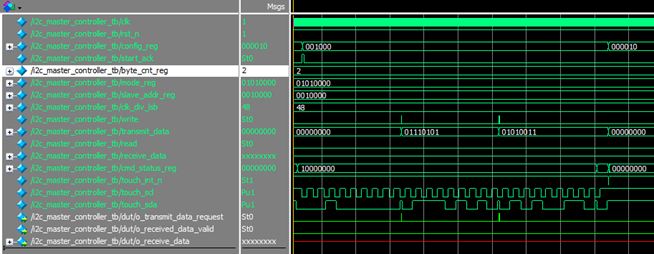
\includegraphics[width=0.95\textwidth,keepaspectratio]{figures/i2c_from_docx/waveform_write.png}
    \caption{Master Transmit — handshake TX}
    \label{fig:w_tx}
\end{figure}

Trong Hình \ref{fig:w_tx}, các tín hiệu điều khiển chính cần đối chiếu theo thứ tự thời gian:
\begin{itemize}[leftmargin=1.2cm]
    \item CPU ghi \texttt{config\_reg} để kích START (quan sát \texttt{start\_ack} và/hoặc bit START tự xóa sau khi bus nhận).
    \item \texttt{byte\_cnt\_reg} xác định số byte truyền; \texttt{slave\_addr\_reg} và mode/prescale quyết định chu kỳ SCL.
    \item Trong khi bus đang chạy, \texttt{o\_transmit\_data\_request} (hoặc \texttt{transmit\_data\_request}) tạo handshake yêu cầu nạp byte TX kế tiếp; dữ liệu ở \texttt{i\_transmit\_data} cập nhật tương ứng.
    \item Sau byte cuối, \texttt{cmd\_status\_reg} chuyển trạng thái (ví dụ TX\_DONE), đồng thời bus quay lại idle sau STOP.
\end{itemize}

\begin{figure}[H]
    \centering
    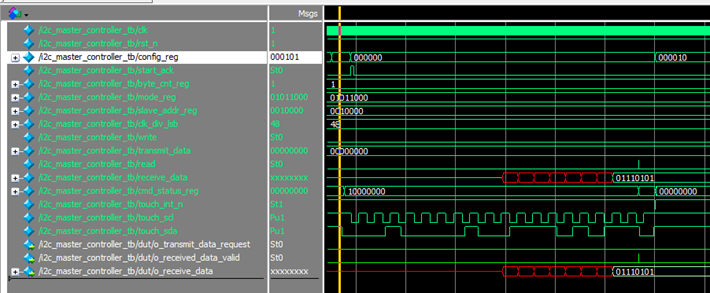
\includegraphics[width=0.95\textwidth,keepaspectratio]{figures/i2c_from_docx/waveform_read.png}
    \caption{Master Receive — data valid và RX\_DONE}
    \label{fig:w_rx}
\end{figure}

Trong Hình \ref{fig:w_rx}, dữ liệu nhận xuất hiện trên \texttt{o\_receive\_data} đồng thời \texttt{o\_received\_data\_valid} lên mức 1 trong cửa sổ hợp lệ. Byte được giữ ổn định để CPU đọc; sau byte cuối, trạng thái hoàn tất (RX\_DONE) được set trong \texttt{cmd\_status\_reg}.

\begin{figure}[H]
    \centering
    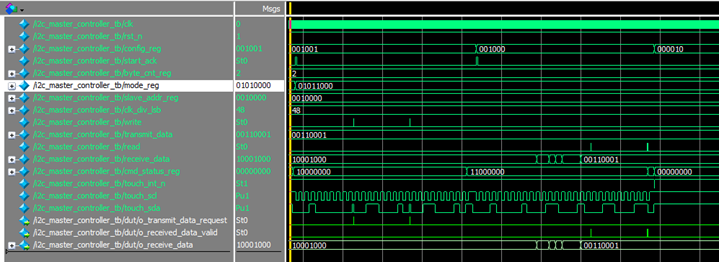
\includegraphics[width=0.95\textwidth,keepaspectratio]{figures/i2c_from_docx/waveform_repeat_start.png}
    \caption{Repeated START (Sr)}
    \label{fig:w_rs}
\end{figure}

Hình \ref{fig:w_rs} thể hiện hai pha giao dịch nối tiếp nhau với \textbf{Repeated START} ở giữa: đường bus không có STOP xen kẽ; sau Sr, địa chỉ/slave phase tiếp theo bắt đầu ngay. Đây là điểm cần kiểm để phân biệt Sr với STOP+START.

